\documentclass[12pt]{article}
\usepackage[utf8]{inputenc}
% \usepackage[english]{babel}
%\usepackage{helvet}
\usepackage{graphicx}
\usepackage{hyperref}
\usepackage{natbib}
\usepackage[inline, shortlabels]{enumitem}
\RequirePackage[a4paper,top=3.5cm,left=3cm,right=3cm,bottom=2.4cm]{geometry}
\title{Fair Price Discovery with Decentralized Exchange}
\author{Yehuda Jay Berg \\jaybny@gmail.com}
\date{May 2021}

\begin{document}
\parindent 0cm
\parskip   6pt
\maketitle

% \documentclass[a4paper]{article}

% \setlength\parindent{0pt}

% \begin{document}

% \title{Sidepit}
% \maketitle
\begin{abstract}
\textbf
\textbf{Ever }since  Satoshi  solved  peer  to  peer  digital  cash  with  Bitcoin,  people have  been  trying  to  apply  similar  techniques  to  solve  other  hard  problems. One such problem, peer to peer exchange, is one of the most difficult of these problems. An exchange is a financial market, where trading of securities occur. The purpose of an exchange is two fold;  1) for price discovery, 2) for counterparty settlement. Centralized Exchanges, have been well researched and developed in traditional finance for well over a century.  They evolved from trading under a tree, to the Chicago trading pits, to electronic exchanges with continuous limit order books. Modern exchanges provide 24/7 trading, and offer co-location for the most prolific traders, high frequency trading bots. Other decentralized exchanges aim to bring traditional centralized exchanges into a peer to peer blockchain protocol. Due to early bitcoin exchange hacks most research has been focused on the settlement utility of exchange. We focus on the price discovery utility, an emergent property of real-time trading. We present fair price discovery with decentralized exchange by solving the impossible task of consensus on total ordering of transactions to mitigate front-running.
\end{abstract}

\section{Introduction}
Ever since Satoshi solved peer to peer digital cash with the Bitcoin protocol, people have been trying to apply similar techniques to other hard problems. Peer to peer decentralized exchange (DEX), is one of the most difficult of these problems. 

The purpose of an exchange in financial markets, is to first match buyers and sellers of financial assets at a \emph{market} price, and then to provide settlement to mitigate any counterparty risk. Tradition electronic exchanges are designed with the goal of reaching a  \emph{price discovery} equilibrium \cite{francioni_schwartz_2017}. Centralized exchanges (CEXs), employ continuous limit order books as a price discovery mechanism. 

Due to well known centralized exchange hacks, coupled with the technical difficulty of decentralized limit order books, most DEXs are solely focused on the non-custodial settlement, rather than \emph{price discovery}. 

\paragraph*{Price discovery} is a social benefit and a key goal in the design of a market structure. In fact, the goal of the architecture of an exchange mechanism, is to attract as much liquidity needed to for price discovery.  \cite{francioni_schwartz_2017}

Price discovery is described in microstructure research as a search for an equilibrium price based on new external information. This new information is reflected in the traders orders, and is ultimately converted into a market price. \citep{RePEc:nbr:nberwo:6257}

Some even define an exchange as ``any trading facility that has as its primary function the delivery of good price discovery'' \cite{francioni_schwartz_2017}. 

However, the price discovery function of an  exchange typically receives insufficient attention in market structure discussions. This is largely attributable to the non-observability of equilibrium prices and, therefore, to the difficulty of quantifying the deviations of transaction prices from their equilibrium values \cite{francioni_schwartz_2017}


\begin{quote}
Price discovery is dynamic in nature, and an efficient price discovery process is characterized by the fast adjustment of market prices from the old equilibrium to the new equilibrium with the arrival of new information \cite{RePEc:udb:wpaper:uwec-2005-01-r}    
\end{quote}

\paragraph*{Limit order books} and price discovery are tightly related. \citep{RePEc:nbr:nberwo:6257} \cite{RePEc:eee:jfinec:v:17:y:1986:i:1:p:5-26}

To achieve price discovery exchanges offer two order types. Limit orders, and Market orders. All orders are sent to a centralized matching engine in the exchange servers. 

Market orders have a quantity but no price. 

\begin{enumerate*}
    \item "Buy 1 @ market" - an order to buy 1 unit of the asset at the market  
\end{enumerate*}

Limit orders have a quantity and a price. 

\begin{enumerate*}
    \item "Buy 1 @ 100" - an order to buy 1 unit of the asset at the market  
\end{enumerate*}


\paragraph*{Continuous limit order book (CLOB)}is the market micro structure that leads to price discovery \footnote{Other types of markets such as call auctions, and dealer markets, do not provide the robustness of limit orders for price discovery. \cite{RePEc:hal:journl:hal-00459785}}. There are two order types. Limit orders, where you provide your own price, with the risk of waiting to be matched and market-orders, where you get filled immediately in return for a possibly worse price.

The interaction where market orders match limit orders is continuous. 

The state of a CLOB in a centralized exchange is shown to produce a price discovery equilibrium. 

The design of CLOB evolved from previous exchanges, futures trading pits in Chicago allowed for price discovery to emerge. 

For the purpose of price discovery, the match of buyers and seller must be atomic, or one party can pull out of the deal after the fact. 


\subsubsection*{Evolution of Exchange}
The design of CLOB evolved from previous exchanges. Futures trading pits in Chicago reached price discovery equilibrium.  

Before electronic markets, an open outcry system in physical trading pits were setup at the exchange place. Buyers and sellers would be bunched up in close proximity to each other, and they would verbalize their intention to buy or sell, the quantity they wish to trade, and the price they are willing to accept or pay. Traders would seek out the best prices by verbally filling with their counterparties. 

\textbf{A match in a trading pit is the real atomic swap} 

For the purpose of Price Discovery what needs to be atomic is the  match, otherwise one party can pull out of the deal. CME provides this guarantee. 

\textbf{Atomic swap DEXs, that allow one side to back out does not provide price discovery.}

Backing out of a trade is the most used move by participants in modern exchanges. In fact, 60\%  of all orders placed on centralized exchanges are cancelled within 1 millisecond. \cite{notsure}  

Going electronic, exchanges were faced with asynchronous message over IP. No longer can buyers and sellers interact simultaneously. Market makers in NASDAQ and specialist in NYSE were tasked with providing liquidity and filling orders. 

Exchanges added anti-front-running rules, so for profit MMs did not abuse the system. Rules, such as Reg NMS were made, not to prevent front-running, 
but to ensure price discovery. \cite{notsure} 

Early market maker based electronic exchanges, such as NASDAQ, were facing problems analogous to the problem of Miner Extracted Value (MEV) we see in Ethereum today. Where miners not only can front-run but they can add their own orders in after seeing everyone elses. Exchanges feared this would lead to loss of confidence in the market which would affect the fragile state where the equilibrium of price discovery exists. 

When designing a DEX, we keep in mind how obvious unfairness will ultimately hurt liquidity, the exchange overall and Price Discovery in particular. In fact, the main issue with decentralized LOB is not the MEV or front-running, but the loss of confidence stemming from those problems.  



\subsubsection*{The HFT Problem}
\textbf{The reason 60\% of all ordes are immediatly canceled in todays markets is due to Continuous Limit Order Books (CLOBs).}

At the turn of the 20th century, exchanges adopted CLOB. No more front-running or market-makers. They were replaced with High Frequency Market Makers (HFT-MM) 

High Frequency refers to the reaction time of automated trading bots. This reaction time determines how often you are incentiviced to cancel your orders. 

Unless you are the absolute fastest, you are incentivized to immediately cancel your market making orders due to \emph{Adverse Selection Risk } (ASR)  

Example: \( reaction time = 2 seconds \) 

$t_0$ limit buy 1 \$IBM @ 100 \\
$t_2$ IBM files bankruptcy 

At $t_0$ you place limit order to buy 1 share of IBM at \$100, and at $t_2$ you learn that IBM has filed bankruptcy, and you immediately cancel. However at $t_2$ your adversary also hears the news, and sends a sell order to attempt to fill you. Its a classic race, fill vs cancel.

$t_2$ hero send cancel order to exchange  \\
$t_2$ villan send sell 1 \$IBM @ market  

Since the villans reaction time is only 1 second while yours is 2 seconds, his orders hits the matching engine at $t_3$ , while Heros cancel doesnt get there until $t_4$. Hero ends up buying IBM after learning they filed bankruptcy! This is an example of \emph{Adverse Selection Risk} (ASR). In fact, all limit orders sitting on the book are subject to ASR. Special \emph{HFT Bandit} bots, are designed just to snip these "stale" limit orders. 

$t_0$ limit buy 1 \$IBM @ 100 \\
$t_1$ cancel \\
$t_2$ if ( no bad news ) limit buy 1 \$IBM @ 100 \\
$t_3$ cancel 

If instead your trading plan was to \emph{flash} all your orders, by sending and immediately canceling. You would have already canceled at $t_1$ and after learning about the bankruptcy, you wouldn't have sent the new buy order at $t_2$

The objective of the Market Maker is to buy at bid and sell at ask over and over again. An adversary reacting faster than them, on the news of an IBM bankruptcy, is an example of ASR . 

Reducing ASR has lead to a massive HFT arms race \cite{notsure} leaving only a handful of players left, till this day. HFT players pay exchanges co-location fees to be as close to the matching engine as possible. 

While \emph{flashing} orders is a defensive move done by even the second fastest bot it is still not as destructive as front-running when it comes to interfering with the price discovery mechanism. 

HFT bots today can only \emph{front-run} public news and data, while old school specialists got to \emph{front-run} their adversaries orders. 

\paragraph{Adverse Selection} (AS) has been well studied and defined in relation to traditional centralized exchange trades. \emph{AS} is when their order to buy, sell, or cancel is only executed when its not in your best interest, and is never filled, when there is a clear profit. 

Numerical models suggest that cancellations is the optimal strategy to avoid \emph{AS}, and that cancelling and reinserting the same order is an optimal implementation. \cite{Lehalle}  Empirical evidence confirms that almost half of all cancellations are resubmitted within one millisecond. \cite{Menkveld2} 

Prior work also shows how speed is directly related to profits by reducing \emph{AS} \cite{Lehalle},  and the profitable response times is in the order of microseconds. \cite{Menkveld2} 

\paragraph{Information Technology:} In addition to speed, HFT make profits from information technology, by modeling the order imbalances of the large institutions. Studies show the overall market-quality improves when \emph{HFT} profits from being informed, and declines when they profit from speed. \cite{Menkveld2}

>>>> How did someone measure quality when we cannot say what the true price is in a given secnod? Seems like there were a lot of assumptions made. Not sure we want to dig in to this but that's what's comes to my mind when reading it <<<<<<<

 
\subsection*{Blockchain DEX Problems}

With decentralized limit order books, \emph{HFT Bots} can now front-run like the old school specialist by reacting to adversarial orders and jumping ahead. 

DEXs with CLOB cannot enforce the anti front-running rules, seen in early electronic exchanges, which kills liquidity and price discovery. 

DEXs cant prevent front-running, because decentralized consensus in limit order books require consensus on total ordering of transactions within blocks on a blockchain. 


\subsubsection*{Front-Running and Permissioned Blockchains}
Front-running is when an adversary sees an honest transaction on the network, and based on that information creates a new transaction in an attempt to beat the original transaction to processing. See Figure \ref{fig:front-running}

Blockchains by design are decentralized with asynchronous transactions, meaning even honest nodes will sometimes receive transactions in different orders. So when a protocol is \emph{order dependent}, front-running attacks are possible.

\begin{figure}[ht]
  \centering 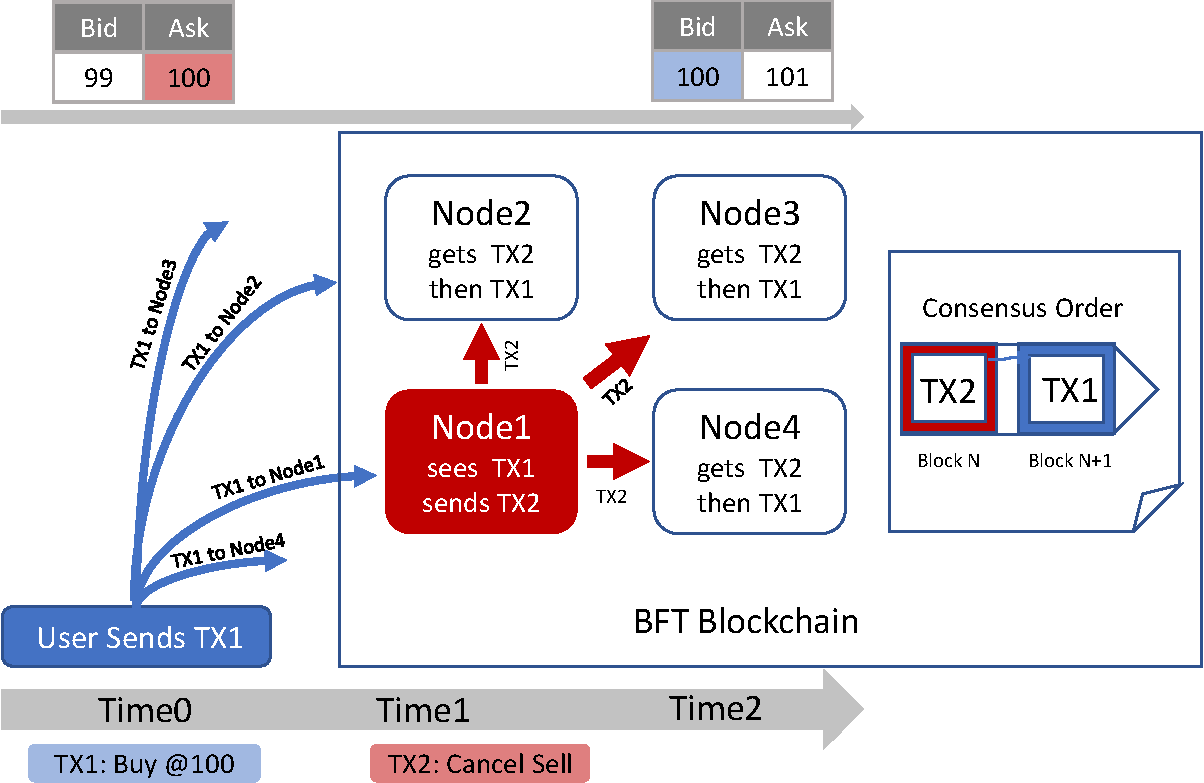
\includegraphics[scale=0.4]{frontrunning3-crop.pdf}
  \caption{Frontrunning in BFT Blockchain - Node1 reads the Users Transaction - \emph{TX1}, and Front runs them with \emph{TX2}, creating \emph{Adverse Selection Risk} for the User}\label{fig:front-running}
\end{figure}


\subsubsection*{MEV and Public Blockchains}
\subsubsection*{Transaction Ordering}
\subsubsection*{Why does it not work?}
\subsection*{New Blockchain Abstraction}

\section{Fair Price Discovery} 

\subsection{Decentralized Limit Order Books}
We start with a closed network of exchange nodes, where each node has a matching-engine and maintains a CLOB, like a centralized exchange. 

The distributed network of nodes come to consensus on the total ordering of transactions. This is done in two steps: 

\begin{enumerate}
    \item \emph{block-data} consensus is reached every N seconds on the full list of transactions from the mempool. 
    \item \emph{block-order} consensus is reached via auction on each block, where the highest bidder gets to reorder the transactions in the \emph{block-data} 
\end{enumerate}

From these two simple steps we have removed the advantage of HFT co-location, the need to front-run and overt \emph{Miner Extracted Value} (MEV) through manipulation of ordering or inclusion of transactions.

\paragraph*{HFT Co-location} is no longer possible as there is no single location for the matching engine. Furthermore, the notion of \emph{being first} goes away, as all orders within the block are the same in regards to time. Also, since you can pay to \emph{be first}, after the fact, there is no longer justification of cost of the HFT arms race. 

\paragraph*{Front-running} by \emph{rushing} has no advantage, as the processing order is not determined by which transaction was seen first on the network. 

\paragraph*{Miner Extracted Value} is no longer possible, as we come to consensus on the entire mempool, for each block. Recall, that \emph{MEV} is defined as a miner choosing, ordering or adding new transactions into a block in a way that generates economic value.  In our model, each block contains all the outstanding transactions, and the transactions in \emph{block-data} are in no particular order for processing, until after the \emph{block-order} auction. 

 
\newpage
\bibliography{sidepit}{}
\bibliographystyle{plain}
% \bibliographystyle{unsrt}

\end{document}